\subsection{FUNCTORIAL PROPERTIES OF THE TENSOR ALGEBRA}

PROPOSITION 2. Let A be a commutative ring, M and N two A-modules and

\[
u: \mathbf {M} \rightarrow \mathbf {N}
\]

an A-linear mapping. There exists one and only one A-algebra homomorphism

\[
u ^ {\prime}: \mathsf {T} (\mathbf {M}) \rightarrow \mathsf {T} (\mathbf {N})
\]

such that the diagram

\pandocbounded{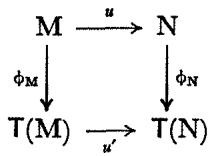
\includegraphics[keepaspectratio]{images/part003_fafbfb88.jpg}}

is commutative. Further, \(u'\) is a graded algebra homomorphism.

The existence and uniqueness of \(u'\) follow from no. 1, Proposition 1, applied to the algebra \(T(N)\) and the linear mapping \(\phi_N \circ u: M \to T(N)\) ; as

\[
u (\mathbf {M}) \subset \mathsf {T} ^ {1} (\mathbf {N}) = \mathbf {N},
\]

the fact that \(u'\) is a graded algebra homomorphism follows from the Remark of no. 1.

The homomorphism \(u'\) of Proposition 2 will henceforth be denoted by \(T(u)\) . If \(P\) is an A-module and \(v: N \to P\) an A-linear mapping, then

\[
\mathsf {T} (v \circ u) = \mathsf {T} (v) \circ \mathsf {T} (u)\tag{4}
\]

for \(\mathsf{T}(v)\circ \mathsf{T}(u)\) is an algebra homomorphism rendering commutative the diagram

\pandocbounded{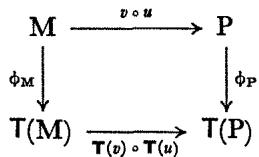
\includegraphics[keepaspectratio]{images/part003_f792dba1.jpg}}

\(\mathsf{T}(u)\) is sometimes called the canonical extension of u to \(\mathsf{T}(\mathbf{M})\) (which contains \(\mathbf{M} = \mathsf{T}^1(\mathbf{M})\) ). Note that the restriction \(\mathsf{T}^n(u): \mathsf{T}^n(\mathbf{M}) \to \mathsf{T}^n(\mathbf{N})\) is just the linear mapping \(u^{\otimes n} = u \otimes u \otimes \cdots \otimes u\) (n times), for

\[
\mathsf {T} ^ {n} (u) \left(x _ {1} \otimes \dots \otimes x _ {n}\right) = u \left(x _ {1}\right) \otimes \dots \otimes u \left(x _ {n}\right)
\]

since \(\mathsf{T}(u)\) is an algebra homomorphism and \(\mathsf{T}^{1}(u)=u\) ; the restriction \(\mathsf{T}^{0}(u)\) to A is the identity mapping. \(\mathsf{T}^{n}(u)\) is called the n-th tensor power of u.

PROPOSITION 3. If \(u: \mathbf{M} \to \mathbf{N}\) is a surjective A-linear mapping, the homomorphism \(\mathsf{T}(u): \mathsf{T}(\mathbf{M}) \to \mathsf{T}(\mathbf{N})\) is surjective and its kernel is the two-sided ideal of \(\mathsf{T}(\mathbf{M})\) generated by the kernel \(\mathbf{P} \subset \mathbf{M} \subset \mathsf{T}(\mathbf{M})\) of \(u\) .

\(T^{0}(u):T^{0}(M)\rightarrow T^{0}(N)\) is bijective and for every integer n\textgreater0,

\[
\mathbf {T} ^ {n} (u): \mathbf {T} ^ {n} (\mathbf {M}) \rightarrow \mathbf {T} ^ {n} (\mathbf {N})
\]

is surjective, as is seen by induction on \(n\) using II, § 3, no. 6, Proposition 6; the latter proposition also shows, by induction on \(n\) , that the kernel \(\mathfrak{S}_n\) of \(\mathsf{T}^n(u)\) is the submodule of \(\mathsf{T}^n(\mathbf{M})\) generated by the products

\[
x _ {1} \otimes x _ {2} \otimes \dots \otimes x _ {n}
\]

where at least one of the \(x_{i}\) belongs to \(\mathbf{P}\) . This shows that the kernel \(\mathfrak{S} = \bigoplus_{n\geqslant 1}\mathfrak{S}_n\) of \(\mathsf{T}(u)\) is the two-sided ideal generated by \(\mathbf{P}\) in \(\mathsf{T}(\mathbf{M})\) .

If \(u: \mathbf{M} \to \mathbf{N}\) is an injective linear mapping, it is not always true that \(\mathbf{T}(u)\) is an injective mapping (Exercise 1). However, this is true when \(u\) is an injection such that \(u(\mathbf{M})\) is a direct factor of \(\mathbf{N}\) , for then there exists a linear mapping \(v: \mathbf{N} \to \mathbf{M}\) such that \(v \circ u\) is the identity mapping on \(\mathbf{M}\) and therefore

\[
\mathsf {T} (v \circ u) = \mathsf {T} (v) \circ \mathsf {T} (u)
\]

is the identity mapping on \(\mathsf{T}(\mathbf{M})\) , hence \(\mathsf{T}(u)\) is injective and its image (isomorphic to \(\mathsf{T}(\mathbf{M})\) ) is a direct factor of \(\mathsf{T}(\mathbf{N})\) (II, §1, no. 9, Proposition 15). More precisely:

PROPOSITION 4. Let N and P be two submodules of an A-module M such that their sum \(N + P\) is a direct factor in M and their intersection \(N \cap P\) is a direct factor in N and in P. Then the homomorphisms \(\mathsf{T}(\mathbf{N}) \to \mathsf{T}(\mathbf{M})\) , \(\mathsf{T}(\mathbf{P}) \to \mathsf{T}(\mathbf{M})\) and

\[
\mathsf {T} (\mathbf {N} \cap \mathbf {P}) \rightarrow \mathsf {T} (\mathbf {M}),
\]

canonical extensions of the canonical injections, are injective; if \(\mathsf{T}(\mathbf{N})\) , \(\mathsf{T}(\mathbf{P})\) and \(\mathsf{T}(\mathbf{N} \cap \mathbf{P})\) are identified with subalgebras of \(\mathsf{T}(\mathbf{M})\) by means of these homomorphisms, then

\[
\mathsf {T} (\mathbf {N} \cap \mathbf {P}) = \mathsf {T} (\mathbf {N}) \cap \mathsf {T} (\mathbf {P}).\tag{5}
\]

By hypothesis, there exist submodules \(N' \subset N\) and \(P' \subset P\) such that \(N = N' \oplus (N \cap P)\) , \(P = P' \oplus (N \cap P)\) ; then

\[
\mathbf {N} + \mathbf {P} = \mathbf {N} ^ {\prime} \oplus \mathbf {P} ^ {\prime} \oplus (\mathbf {N} \cap \mathbf {P})
\]

and there exists by hypothesis a submodule \(M'\) of M such that

\[
\begin{array}{c} \mathbf {M} = \mathbf {M} ^ {\prime} \oplus (\mathbf {N} + \mathbf {P}) = \mathbf {M} ^ {\prime} \oplus \mathbf {N} ^ {\prime} \oplus \mathbf {P} ^ {\prime} \oplus (\mathbf {N} \cap \mathbf {P}) \\ = \mathbf {M} ^ {\prime} \oplus \mathbf {P} ^ {\prime} \oplus \mathbf {N} = \mathbf {M} ^ {\prime} \oplus \mathbf {N} ^ {\prime} \oplus \mathbf {P}. \end{array}
\]

In particular, \(N + P\) , N, P and \(N \cap P\) are direct factors in M, which implies, as has been seen above, that the canonical homomorphisms

\[
\begin{array}{l} \mathsf {T} (\mathbf {N} + \mathbf {P}) \to \mathsf {T} (\mathbf {M}), \qquad \mathsf {T} (\mathbf {N}) \to \mathsf {T} (\mathbf {M}), \\ \mathsf {T} (\mathbf {P}) \to \mathsf {T} (\mathbf {M}), \qquad \mathsf {T} (\mathbf {N} \cap \mathbf {P}) \to \mathsf {T} (\mathbf {M}) \end{array}
\]

are injective. The three algebras \(\mathsf{T}(\mathbf{N})\) , \(\mathsf{T}(\mathbf{P})\) and \(\mathsf{T}(\mathbf{N} \cap \mathbf{P})\) are thus identified with subalgebras of \(\mathsf{T}(\mathbf{N} + \mathbf{P})\) and the latter with a subalgebra of \(\mathsf{T}(\mathbf{M})\) ;

writing \(\mathbf{Q} = \mathbf{N} \cap \mathbf{P}\) , it remains to show that, if \(\mathsf{T}(\mathbf{Q})\) , \(\mathsf{T}(\mathbf{N}' \oplus \mathbf{Q})\) and \(\mathsf{T}(\mathbf{P}' \oplus \mathbf{Q})\) are identified with subalgebras of \(\mathsf{T}(\mathbf{N}' \oplus \mathbf{P}' \oplus \mathbf{Q})\) , then

\[
\mathsf {T} (\mathbf {N} ^ {\prime} \oplus \mathbf {Q}) \cap \mathsf {T} (\mathbf {P} ^ {\prime} \oplus \mathbf {Q}) = \mathsf {T} (\mathbf {Q}).\tag{6}
\]

Now, consider the commutative diagram

\pandocbounded{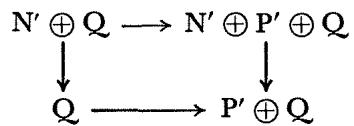
\includegraphics[keepaspectratio]{images/part003_8d12e188.jpg}}

where the horizontal arrows are the canonical injections and the vertical arrows the canonical projections. We derive a commutative diagram

\begin{enumerate}
\def\labelenumi{(\arabic{enumi})}
\setcounter{enumi}{6}
\tightlist
\item
\end{enumerate}

\pandocbounded{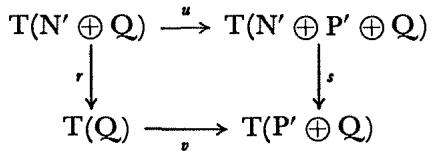
\includegraphics[keepaspectratio]{images/part003_389443db.jpg}}

where r and s are surjective homomorphisms (Proposition 3) and u and v injective homomorphisms. Hence, to prove (6), note that the right hand side is obviously contained in the left; it therefore suffices to verify that if

\[
x \in \mathsf {T} (\mathbf {N} ^ {\prime} \oplus \mathbf {Q}) \cap \mathsf {T} (\mathbf {P} ^ {\prime} \oplus \mathbf {Q}),
\]

then \(x \in \mathsf{T}(\mathsf{Q})\) . Now the definition of the homomorphism s shows that its restriction to \(\mathsf{T}(\mathsf{P}' \oplus \mathsf{Q})\) (identified with a subalgebra of \(\mathsf{T}(\mathsf{N}' \oplus \mathsf{P}' \oplus \mathsf{Q})\)) is the identity mapping; the hypothesis on x therefore implies that \(s(u(x)) = x\) . But then also \(v(r(x)) = x\) , in other words x belongs to the image of \(\mathsf{T}(\mathsf{Q})\) in \(\mathsf{T}(\mathsf{P}' \oplus \mathsf{Q})\) , which was to be proved.

Remark. Note in particular that the hypotheses of Proposition 4 always hold for arbitrary submodules N, P of M when A is a field (II, § 7, no. 3, Proposition 4). Moreover, if N ⊂ P and N ≠ P, then T \(^{n}\) (N) ≠ T \(^{n}\) (P) for all n ≥ 1, since if R is a complement of P in N, then T \(^{n}\) (P) ∩ T \(^{n}\) (R) = \{0\} by (4) and T \(^{n}\) (R) ≠ \{0\}.

COROLLARY. Let K be a commutative field and M a vector space over K. For every element \(z \in \mathsf{T}(\mathbf{M})\) , there exists a smallest vector space N of M such that \(z \in \mathsf{T}(\mathbf{N})\) and N is of finite rank over K.

It is understood in this statement that for every vector subspace P of M, \(T(P)\) is canonically identified with a subalgebra of \(T(M)\) . Let \(z \in T(M)\) ; z can be expressed as a linear combination of elements each of which is a finite product of elements of \(M = T^{1}(M)\) ; all the elements of M which occur in these products generate a vector subspace Q of finite rank and \(z \in T(Q)\) .

Let \(\mathfrak{F}\) be the (non-empty) set of vector subspaces \(\mathbf{P}\) of finite rank such that \(z\in \mathsf{T}(\mathbf{P})\) . Every decreasing sequence of elements of \(\mathfrak{F}\) is stationary, since they are vector spaces of finite rank. Hence \(\mathfrak{F}\) has a minimal element \(\mathbf{N}\) (Set Theory, III, §6, no. 5). It remains to verify that every \(\mathbf{P}\in \mathfrak{F}\) contains \(\mathbf{N}\) ; now, \(z\in \mathsf{T}(\mathbf{P})\cap \mathsf{T}(\mathbf{N}) = \mathsf{T}(\mathbf{P}\cap \mathbf{N})\) (Proposition 4); in view of the definition of \(\mathbf{N}\) , this implies \(\mathbf{N}\cap \mathbf{P} = \mathbf{N}\) , that is \(\mathbf{P}\supset \mathbf{N}\) .

The subspace N of M is said to be associated with z.

